\documentclass[TA.tex]{subfiles}

\begin{document}


%\hyphenation{equi-va-len-cia}\hyphenation{pro-pie-dad}\hyphenation{res-pec-ti-va-men-te}\hyphenation{sub-es-pa-cio}

\chapter{Homología}

Para nociones de homología simplicial, consultar los apuntes de Homología Simplicial. Atención: en homología ordenada no existen los símplices en orden distinto al prefijado, no se toma cociente. 
\section{Homología singular}

Dado un espacio topológico $X$, definimos un $n$-\emph{símplice singular} como una aplicación continua $\sigma_n:\Delta^n\to X$, donde $\Delta^n$ es el $n$-símplice estándar. Denotamos $C_n(X)$ al grupo abeliano libre de todos los $n$-símplices singulares. A las combinaciones de la forma $\sum_{i=1}^n\lambda_i\sigma_n^i$ con $\lambda_i\in\Z$ se las llama $n$-\emph{cadenas} (estos son de hecho todos los elementos de $C_n(X)$. Tenemos definido también el operador borde $d_n:C_n(X)\to C_{n-1}(X)$, que es un homomorfismo de grupos abelianos definido como $d_n(\sigma_n)=\sum_{i=0}^n \sigma_n|_{[v_0,\dots, \hat{v_i},\dots, v_n]}$. Este operador verifica las mismas propiedades que el operador borde entre complejos simpliciales, con idéntica demostración. Así que hemos construido un complejo de cadenas singulares $\{C_n(X), d_n\}_{n\geq 1}=C_*(X)$. En caso de usar coeficientes en un grupo $G$ se indicará como $C_*(X,G)$. Análogamente a la homología simplicial, si $z\in C_n(X)$ y $d(z)=0$, decimos que $z$ es un $n$-ciclo. Si $z=d_{n+1}(z')$ para algún $z'\in C_{n+1}(X)$, decimos que $z$ es un $n$-borde. Como tenemos $B_n(X)=\Ima d_{n+1}\subseteq \ker d_n=Z_n(X)$, definimos el $n$-ésimo grupo de homología singular $H_n(X)=Z_n(X)/B_n(X)$. 


\begin{prop}
Si $X=\sqcup X_i$ (cantidad finita) es una descomposición de $X$ en sus componentes conexas por caminos, entonces $H_n(X)\cong \oplus_i H_n(X_i)$. 
\end{prop}
\begin{dem}
Como un símplice singular siempre tiene imagen conexa por caminos, $C_n(X)$ se escribe como suma directa de $C_n(X_i)$. Como $d_n$ respeta esta descomposición, $\ker d$ e $\Ima d$ se descomponen de la misma forma, por lo que $H_n(X)\cong \oplus_i H_n(X_i)$. \QED
\end{dem}

\begin{prop}\label{2.7}
Si $X\neq\emptyset$ es arco-conexo, entonces $H_0(X)\cong\Z$. 
\end{prop}
\begin{dem}
Por definición $H_0(X)=Z_0(X)/B_0(X)=C_0(X)/Ima d_1$. Definimos una aumentación $\varepsilon:C_0(X)\to\Z$ como $\varepsilon(\sigma_0)=1$ para todo 0-símplice singular. Como $X\neq\emptyset$, $\varepsilon$ es sobreyectivo, porque podemos un el 0-símplice. Vamos a probar que $\ker\varepsilon=\Ima d_1$, con lo que usando el primer teorema de isomorfía tendremos que $H_0(X)\cong \Ima\varepsilon=\Z$. 

Veamos primero $\Ima d_1\subseteq\ker\varepsilon$. Sea $\sigma_1:\Delta^1\to X$, entonces $\varepsilon(d_1(\sigma_1))=\varepsilon(\sigma_1|_{v_1})-\varepsilon(\sigma_1|_{v_0})=0$.

Ahora la inclusión contraria, $\ker\varepsilon\subseteq\Ima d_1$. Sea $z\in C_0(X)$ tl que $\varepsilon(z)=0$. Por definición $z=\sum_{i=1}^k \lambda_i\sigma^i$, donde $\sigma_i$ son aplicaciones constantes $x_i$. Entonces $\varepsilon(z)=\sum_{i=1}^k\lambda_i$. Consideramos los 1-símplices singulares $\tau_i$ que son un camino entre $x_0$ y $x_i$ y definimos $\tau=\sum_{i=1}^k\lambda_i\tau_i\in C_1(X)$. Entonces
\[
d_1(\tau)=\sum_{i=1}^k \lambda_id(\tau_i)=\sum_{i=1}^k \lambda_i(x_i-x_0)=\sum_{i=1}^k\lambda_i\sigma_i-(\sum_{i=1}^k\lambda_i)x_0
\]
Como $\sum_{i=1}^k\lambda_i=0$ por ser $\varepsilon(z)=0$,  $d_1(\tau)=z$. \QED
\end{dem}

\begin{prop}
Si $X$ es un punto, entonces $H_n(X)=0$ para $n>0$ y $H_0(X)=\Z$.
\end{prop}

\begin{dem}
$H_0(X)=\Z$ se tiene por ser $X$ arco-conexo. Para el resto de caso miramos directamente el complejo de cadenas. $C_n(X,\Z)$ tiene solamente un $n$-símplice singular $\sigma_n$, y el operador borde $d(\sigma_n)=\sum_i (-1)^i\sigma_{n-1}$, que es 0 para $n$ impar y $\sigma_{n-1}$ para $n$ par. Entonces tenemos el complejo de cadenas
\[
\cdots\Z\xrightarrow{\cong}\Z\xrightarrow{0}\Z\xrightarrow{\cong}\Z\xrightarrow{0}\Z\to 0
\]
cuya homología es trvial para $n>0$. 
\QED
\end{dem}

Una variación del complejo de cadenas singulares es el complejo de cadenas singulares aumentado, definiendo $\varepsilon:C_0(X)\to \Z$ como $\varepsilon(\sigma_0)=1$ para todo 0-símplice singular. Denotamos como $\widetilde{C}_n$ a los grupos de este complejo, que en realidad coinciden en todos los niveles salvo en -1, que es $\Z$. Hemos visto en la demostración de la proposición \ref{2.7} que $\varepsilon d_1=0$, así que podemos definir la homología reducida con valor
\[
\widetilde{H}_n(X)=\begin{cases}
H_n(X) & n>0\\
H_0(X)/\Z & n=0
\end{cases}
\]
El primer caso es trivial, vamos a probar el segundo, aunque usaremos algunas nociones de álgebra que veremos más adelante.  Tenemos el diagrama conmutativo
\[
\begin{tikzcd}
\ker\varepsilon\arrow[rd,twoheadrightarrow]\arrow[r,twoheadrightarrow] & \ker\overline{\varepsilon}\arrow[r, rightarrowtail]& H_0(X)\arrow[d, twoheadrightarrow, "\overline{\varepsilon}"]\\
C_1(X)\arrow[r, "d_1"]\arrow[d, twoheadrightarrow] & C_0(X)\arrow[r, twoheadrightarrow, "\varepsilon"]\arrow[ur,twoheadrightarrow]  & \Z\\
\Ima{d_1}\arrow[ur, rightarrowtail]
\end{tikzcd}
\]
donde $\overline{\varepsilon}$ es la aplicación inducida en $H_0(X)$ por $\varepsilon$ (es fácil comprobar que está bien definida). El hecho de que $\varepsilon\circ d_1=0$ nos proporciona además $\Ima d_1 \rightarrowtail\ker\varepsilon$. Esto nos da la sucesión exacta corta
\[
\Ima d_1 \rightarrowtail\ker\varepsilon\twoheadrightarrow\ker\overline{\varepsilon}
\]
El primer teorema de isomorfía nos da además $\ker\overline{\varepsilon}\cong \ker\varepsilon/\Ima d_1=\widetilde{H}_0(X)$. Así sustituyendo en el diagrama anterior obtenemos la sucesión exacta corta
\[
\widetilde{H}_0(X)\rightarrowtail H_0(X)\overset{\overline{\varepsilon}}{\twoheadrightarrow}\Z
\]
Como el grupo de la derecha es abeliano libre, la sucesión escinde, con lo que $H_0(X)=\Z\oplus \widetilde{H}_0(X)$.

%$\twoheadleftarrow \twoheadrightarrow \rightarrowtail \leftarrowtail$

\subsection{Invariancia homotópica}

%f_\sharp

Si tenemos una aplicación continua $X\to Y$, se induce una aplicación $f_*: C_n(X)\to C_n(Y)$ definido como $\sigma\mapsto f\circ\sigma$, que conmuta con el operador borde (es un morfismo de complejos de cadenas), como vamos a comprobar.  Si $\sigma\in C_n(X)$, 
\[
f_*(d_n(\sigma))=\sum_{i=0}^n (-1)^i (f\circ\sigma)|_{[v_0,\dots, \hat{v_i}, \dots, v_n]}=d_n(f\circ\sigma)
\]

Esto implica que si $z\in C_n(X)$ con $d(z)=0$, entonces $d_n(f_*(z))=f_*(d_n(z))=0$, por lo que $f_*$ envía ciclos en ciclos. De igual manera, envía bordes en bordes. De este modo, se induce un homomorfismo dentado igual, $f_*:H_n(X)\to H_n(Y)$. 

Además $(g\circ f)_*=g_*\circ f_*$ y $(Id_X)_*=Id_*$ tanto en complejos de cadenas como en homología.


\begin{teorema}
Si $f,g:X\to Y$ son continuas con $f\simeq g$, entonces $f_*=g_*:H_n(X)\to H_n(Y)$ para todo $n\geq 0$. 
\end{teorema}\
 \opencutright
\begin{dem}
%This is where the table goes with text wrapping around it. You may 
%embed tabular environment inside wraptable environment and customize as you like.

%------------------------------------------
%\begin{wrapfigure}{r}{4cm}
%\caption{A wrapped figure going nicely inside the text.}\label{wrap-fig:1}
%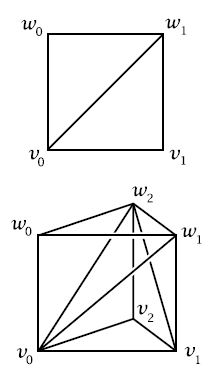
\includegraphics[width=4cm]{cilindrosimplice}
%\end{wrapfigure} 
%------------------------------------------
\def\windowpagestuff{\flushright 
   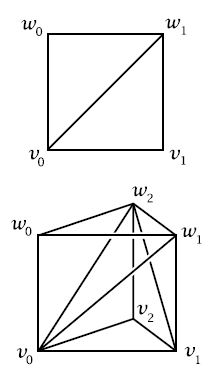
\includegraphics[width=2.8cm,height=4.5cm]{cilindrosimplice}}
   
  
   \begin{cutout}{1}{0.75\textwidth}{0pt}{6}
     \noindent
El primer paso será subdividir $\Delta^n\times I$ en simplices. Sea $\Delta^n\times\{0\}=[v_0,\dots, v_n]$ y $\Delta^n\times\{1\}=[w_0,\dots, w_n]$, donde $v_i$ tiene la misma imagen que $w_i$ mediante la proyección $\Delta^n\times I\to \Delta$. Para cada $0\leq i\leq n$ consideramos el $(n-1)$-símplice $[v_0,\dots, v_i, w_i,\dots, w_n]$. Este símplice se ha conseguido simplemente recorriendo $\Delta^n\times\{0\}$ hasta el vértice $v_i$ y después saltando a $w_i$ para recorrer el resto de $\Delta^n\times\{1\}$, para luego volver a $v_0$. La figura muestra los casos $n=1,2$.
\end{cutout}\
%INTENTAR CON CUTWIN \url{https://tex.stackexchange.com/questions/40806/how-to-wrap-text-around-a-figure-revised}
%\begin{figure}[h!]
%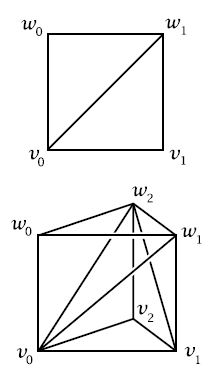
\includegraphics[scale=0.7]{cilindrosimplice}
%\end{figure}

Dada una homotopía $F:X\times I\to Y$ y un símplice singular $\sigma:\Delta^n\to X$, podemos formar la composición $F\circ(\sigma\times Id):\Delta^n\times I\to X\times I\to Y$. Usando esto podemos definir el \emph{operador prisa} $P:C_n(X)\to C_{n+1}(Y)$ como sigue
\[
P(\sigma)=\sum_i(-1)^iF\circ(\sigma\times I)|_{[v_0,\dots, v_i, w_i,\dots, w_n]}
\]
Vamos a demostrar que el operador prisma satisface la relación
\[
dP=g_*-f_*-Pd
\]
Para probarlo calculamos
\[
dP(\sigma)=\sum_{j≤i}
(−1)^i(−1)^jF\circ(σ \times Id)|_{ 
[v_0, \dots, \hat{v}_j , \dots ,v_i,w_i, \dots ,w_n]}
+\sum_{j≥i}
(−1)^i(−1)^{j+1}F\circ(σ\times Id)|_{
[v_0, \dots ,v_i,w_i, \dots ,\hat{w}_j , \dots ,w_n]}
\]
Los términos para $i=j$ se cancelan excepto para $F\circ(σ \times Id)|_{ 
[\hat{v}_0,w_0,\dots ,w_n]}$, que es $g\circ\sigma=g_*(\sigma)$; y $-F\circ(σ \times Id)|_{ 
[v_0,,\dots ,v_n,\hat{w}_n]}$, que es $-f\circ \sigma=-f_*(\sigma)$. Los términos para $i\neq j$ son exactamente $-Pd(\sigma)$. 

Así, si $\alpha\in Z_n(X)$, entonces $g_*(\alpha)-f_*(\alpha)=Pd(\alpha)+dP(\alpha)=dP(\alpha)$ por ser $d\alpha=0$. Entonces $g_*(\alpha)$ y $f_*(\alpha)$ determinan la misma clase de homología al ser su diferencia un borde. 
%Para el caso aumentado creo que P=0 (comprobar).
\end{dem}

En la prueba hemos usado la relación $dP-Pd=f_*-g_*$, que es la que define una \emph{homotopía de complejos de cadenas} entre $f_*$ y $g_*$ (se denota en ese caso $f_*\simeq g_*$). Una \emph{equivalencia de homotopía} enre complejos de cadenas $f:C_*\to D_*$ es un morfismo de complejos de cadenas tal que existe $g:D_*\to C_*$ de modo que $g\circ f\simeq Id_{C_*}$ y $f\circ g\simeq Id_{D_*}$.  Hemos probado además que una equivalencia de homotopía de complejos de cadenas induce isomorfismo en la homología. Para el caso de homología reducida también es válido este resultado definiendo $f_*:\Z\to\Z$ como 0 y $P:\Z\to C_0(Y)$ como la aplicación nula.

\begin{coro}
Si $f:X\to Y$ es equivalencia homotópica, entonces $f_*$ es isomorfismo.
\end{coro}

\section{Álgebra Homológica}

Asumimos conocidas las definiciones y propiedades básicas de las sucesiones exactas. 

\begin{lemma}[Splitting lemma]
Dada una sucesión exacta de módulos $0\to A\xrightarrow{f}B\xrightarrow{g}C\to 0$ son equivalentes:
\begin{enumerate}[a)]
\item Hay un morfismo $p:B\to A$ tal que $pf=Id:A\to A$.
\item Hay un morfismo $s:C\to B$ tal que $gs=Id:C\to C$. 
\item Existe un isomorfismo $B\cong A\oplus C$ compatible con la sucesión exacta corta, es decir, que hace conmutar el siguiente diagrama
\[
\begin{tikzcd}
A\arrow[r, rightarrowtail, "f"]\arrow[d, equals] & B\arrow[r, twoheadrightarrow, "g"]\arrow[d, "u"] & C\arrow[d, equals] \\
A\arrow[r, "i"] & A\oplus C\arrow[r, "\pi"]& C
\end{tikzcd}
\]
\end{enumerate}
\end{lemma}
\begin{proof}
Que c) implica a) y b) es trivial.

Para ver que a) implica c), sea $p:B\to A$ un homomorfismo que verifique $pf=Id$. En este caso, afirmamos que $B=f(A)\oplus\ker p$. Si $b\in B$, entonces $b=fp(b)+(m-fp(b))$. Es claro que $fp(b)\in f(A)$ y además $p(b-fp(b)=p(b)-pfp(b)=p(b)-p(b)=0$, luego $b-fp(b)\in\ker p$. Se tiene también que si $b\in f(A)\cap\ker p$, entonces $b=f(a)$ y $0=p(b)=pf(a)=a$, por lo que $b=0$, con lo que la afirmación es cierta. Una vez que tenemos $b=f(a)+b'$, definimos el homomorfismo $u(b)=a+g(b')$. Se tiene de hecho que $u(b)=a+g(b)$, pues si $b-b'=f(a)$ y por exactitud $g(b-b')=0$. Esta definición no es ambigua por ser $f$ inyectiva. Por la definición que se ha hecho, el diagrama es conmutativo y el lema de los 5 implica que $u$ es isomorfismo.

Por último veamos que b) implica c). Sea $s:C\to B$ tal que $gs=Id$. Afirmamos que $B=\ker g\oplus s(C)$. Sea $b\in B$, lo escribimos como $b=(b-sg(b))+sg(b)$. Es claro que $sg(b)\in s(C)$ y además $g(b-sg(b))=g(b)-gsg(b)=g(b)-g(b)=0$, por lo que $b-sg(b)\in\ker g$. Si $b\in\ker g\cap s(C)$, entonces $b=s(c)$ y $0=g(b)=gs(c)=c$, por lo que $b=0$, lo que prueba la afirmación. Ahora, como $\ker g=\Ima f$, podemos expresar $b=f(a)+s(c)$. Definimos entonces $u(b)=a+c$, lo cual tiene sentido porque tanto $f$ como $s$ son inyectivas y además $\Ima s\cap\Ima f=\Ima s\cap\ker g=0$. La definición que hemos hecho hace conmutar el diagrama y esto hace que $u$ sea isomorfismo por el lema de los cinco. 
\end{proof}

Cuando $C$ es un objeto proyectivo se verifica la escisión. En particular, cuando sea un objeto libre. Se recuerda que una sucesión de complejos  de cadenas $0\to A^*\to B^*\to C^*\to 0$ se dice exacta si lo es en cada nivel. Se advierte que el hecho de que se tenga escisión en cada nivel no implica que $B^*\cong A^*\oplus C^*$ pues los isomorfismos de cada nivel no tienen por qué ser compatibles con el operador borde. 

\begin{teorema}
Toda sucesión exacta corta de complejos de cadenas $0\to A\xrightarrow{f} B\xrightarrow{g} C\to 0$ induce una sucesión exacta larga
\[
\cdots \to H_n(A)\xrightarrow{f_*}H_n(B)\xrightarrow{g_*}H_n(C)\xrightarrow{\partial}H_{n-1}(A)\to\cdots
\] 
%\xrightarrow[g] pone la g debajo
\end{teorema}
La prueba sigue la clásica estrategia de \emph{diagram chasing} y se puede encontrar a partir de la página 116 de \emph{Algebraic Topology} de Allen Hatcher. 
\section{Homología relativa}

Dado un subespacio $A\subseteq X$, vamos a construir el complejo de cadenas relativo $C_*(X,A)$ asociado al par $(X,A)$, lo que nos dará la homología relativa $H_*(X,A)$. Esto se consigue definiendo $C_n(X,A)=C_n(X)/C_n(A)$. Este cociente tiene sentido porque $A\subseteq X$ y entonces el complejo está contenido mediante la aplicación inducido por la inclusión. Como $d$ lleva $C_n(A)$ en $C_{n-1}(A)$, podemos definir $d:C_n(X,A)\to C_{n-1}(X,A)$ como $d([x])=[d(x)]$. Así, la homología relativa es la homología del complejo de cadenas $H_n(X,A)=H_n(C_*(X,A))$. 

A partir de las sucesión exacta corta evidente $0\to C_*(A)\to C_*(X)\to C_*(X,A)\to 0$ surge la sucesión exacta larga de homología relativa
\[
\cdots \to H_n(A)\xrightarrow{f_*}H_n(X)\xrightarrow{g_*}H_n(X,A)\xrightarrow{\partial}H_{n-1}(A)\to\cdots
\]

\begin{defi}
Una aplicación de pares $f:(X,A)\to (Y,B)$ es una aplicación $f:X\to Y$ tal que $f(A)\subseteq B$. 
\end{defi}

Una aplicación de pares induce una aplicación $f|_A:A\to B$, así que se puede definir un morfismo de complejos de cadenas inducido por $f$, $f_*:C_*(X,A)\to C_*(Y,B)$ como $[c]\mapsto [f_*(c)]$ que cumple las propiedades de funtorialiad. Por tanto da lugar también a un homomorfismo en homología $f_*:H_*(X,A)\to H_*(Y,B)$, que es natural con respecto a la sucesión exacta larga de homología relativa, es decir, conmuta el diagrama 
\[
\begin{tikzcd}
\cdots \to H_n(A)\arrow[r]\arrow[d, "f|_{A*}"] & H_n(X)\arrow[r]\arrow[d, "f_*"] & H_n(X,A)\arrow[d, "f_*"]\arrow[r] &H_{n-1}(A)\arrow[d]\to\cdots\\
\cdots \to H_n(B)\arrow[r] & H_n(Y)\arrow[r] & H_n(X,B)\arrow[r]& H_{n-1}(B)\to\cdots
\end{tikzcd}
\]

ya que la conmutatividad se tiene ya a nivel de complejos de cadenas, y la conmutatividad con $\partial$ se puede probar. 
 

\begin{teorema}[de excisión]\label{excision}
Sean subespacios $Z\subseteq A\subseteq X$ tal que la clausura de $Z$ está en el interior de $A$. Entonces la inclusión $i:(X-Z,A-Z)\hookrightarrow (X,A)$ induce isomorfismos $i_*:H_n(X-Z,A-Z)\to H_n(X,A)$ para todo $n$. Equivalentemente, para subespacios $A,B\subseteq X$ cuyos interiores cubren $X$, la inclusión $(B,A\cap B)\hookrightarrow (X,B)$ induce isomorfismos $H_n(B,A\cap B)\to H_n(X,B)$ para todo $n$. 
\end{teorema}

Para un espacio $X$, consideremos una familia de subconjuntos $\mathcal{U}=\{U_i\}_{i\in I}$ tales que $X=\cup_i int(U_i)$. Decimos que un símplice singular en $X$, $\sigma:\Delta^n\to X$ está \emph{subordinado} a $\mathcal{U}$ si existe $I\in I$ con $\delta(\Delta^n)\subseteq U_i$. Denotamos $C^{\mathcal{U}}_*$ al complejo de cadenas de símplices de $X$ subordinados a $\mathcal{U}$, que está contenido en $C_*(X)$.  El operador borde está bien definido, puesto que si $\sigma:\Delta^n\to X$ es tal que $\sigma(\Delta^n)\subseteq U_i$ y si $\Delta^n_i$ es la $i$-ésima cara de $\Delta^n$, entonces $d(\sigma)=\sum_{i=0}^n(-1)^i\sigma|_{\Delta^n_i}$. Como $\sigma(\Delta^n)\subseteq U_i$, también lo está la restricción a cada una de las caras.

\begin{teorema}[de las cadenas pequeñas]\label{peque}
La inclusión $C^{\U}_*(X)\hookrightarrow C_*(X)$ es una equivalencia homotópica de complejos de cadenas. 
\end{teorema}

\begin{defi}
El \emph{baricentro} de un símplice $\sigma=[v_0,\dots, v_n]$ es $b(\sigma)=\sum_{i=0}^n\frac{1}{n+1}v_i\in \sigma$. La \emph{subdivisión baricéntrica} es el complejo simplicial formado por los baricentros de las caras de $\sigma$. La $k$-ésima subdivisión baricéntrica es la división baricéntrica de la $k-1$-ésima subvidisión baricéntrica.
\end{defi}

En general, si $\sigma$ es un símplice y dados $\sigma_0\leq\cdots\sigma_t\leq\sigma$, se tiene que $[b(\sigma_0),\dots, b(\sigma_t)]$ forma un símplice contenido en $\sigma$. 

Se define el \emph{diámetro} de $\sigma\subseteq \R^N$ como $dia(\sigma)=\max_{x,y\in\sigma} d(x,y)$. Denotamos $d(x,y)$ como $|x-y|$. Dados $x,y\in\sigma$, con $y=\sum_{i=0}^n t_iv_i$ y $\sum_{i=0}^nt_i=1$, 
\[
|x-y|=\left|\sum_{i=0}^nt_ix-\sum_{i=0}^nt_iv_i\right|=\left|\sum_{i=0}^nt_i(x-v_i)\right|\leq \sum_{i=0}^n t_i|x-v_i|\leq \sum_{i=0}^nt_i\max_{j=0,\dots, n}|x-v_j|=\max|x-v_j|\leq \max|v_k-v_j|
\]

\begin{lemma}
 Si $\tau$ es un símplice de la subdivisión baricéntrica de $\sigma$, $\dim(\sigma)=n$, 
\[
dia(\tau)\leq\frac{n}{n+1}dia(\sigma)
\]
\end{lemma}

La demostración se puede encontrar en los apuntes de Homología Simplicial o alternativamente en Hatcher página 120. 

\begin{coro}
Si $\tau$ es un símplice de la $k$-ésima subdivisión baricéntrica de $\sigma$, $\dim(\sigma)=n$, 
\[
dia(\tau)\leq \left(\frac{n}{n+1}\right)^k dia(\sigma)
\]
\end{coro}

\begin{coro}\label{r}
Sea $\sigma$ un $q$-símplice sobre $X$ y $\mathcal{P}$ un recubrimiento por abiertos de $X$. Entonces $\exists r>0$ tal que $S^r(\sigma)$ es combinación lineal de símplices subordinados a $\mathcal{P}$, esto es, si $\mathbb{P}=\{V_i\}_{i\in I}$, existe $i\in I$ con $\Ima\sigma\in V_i$. 
\end{coro}
\begin{dem}
$\sigma$ es una aplicación continua que parte de un espacio métrico compacto, luego $\{\sigma^{-1}(V_i)\}$ es recubrimiento de $\Delta^q$. Tomamos $\varepsilon>0$ el número de Lebesgue de $\Delta_q$ respecto de $\sigma^{-1}(\mathcal{P})$. Entones existe $r>0$ tal que el diámetro de $S^r(\Delta_q))$ es menor que $\varepsilon$, por lo que $S^r(\sigma)$ está subordinado a $\mathcal{P}$. 
\end{dem}

\begin{dem}[del teorema de Excisión]
No usamos la estrategia de Hatcher sino de Greenberg, usando que $C_*^{\UU}(X,A)\to C_*(X,A)$ induce isomorfismo en homología. Definimos un morfismo de complejos de cadenas $S:C_q(X)\to C_q(X)$ llamado \emph{subdivisión} y una homotopía de complejos de cadenas $T:C_*(X)\to C_{*+1}(X)$ entre la identidad y $S$, es decir $dT+Td=Id-S$, que funcionarán de forma natural (como functores). En particular, si $\sigma:\Delta^q\to X$, tenemos el diagrama conmutativo
\[
\begin{tikzcd}
C_q(\Delta^q)\arrow[r, "S_q"]\arrow[d, "\sigma_*"] & C_q(\Delta^q)\arrow[d, "\sigma_*"]\\
C_q(X)\arrow[r, "S_q"] & C_q(X)
\end{tikzcd}
\] 
Si consideramos la identidad $\delta:\Delta^q\to\Delta^q\in C_q(\Delta^q)$, $\sigma=\sigma_*(\delta)\in C_q(X)$, entonces $S_q(\sigma)=\sigma_*(S_q(\delta))$. 

Tendremos luego un cubo como el siguiente 
\[
\begin{tikzcd}
&
C_q(\Delta^q)
\ar{dl}[swap, sloped, near start]{\sigma_*}
\ar{rr}{S_q}
\ar[]{dd}[near start]{d}
& & C_q(\Delta^q)
\ar{dd}{d}
\ar{dl}[swap, sloped, near start]{\sigma_*}
\\
C_q(X)
\ar[crossing over]{rr}[near end]{S_q}
\ar{dd}[swap]{d}
& & C_{q}(X)
\ar[crossing over]{dd}[]{d}
\\
&
C_{q-1}(\Delta^q)
\ar[near start]{rr}{S_{q-1}}
\ar[sloped, swap]{dl}{\sigma_*}
& & C_{q-1}(\Delta^q)
\ar[sloped, swap]{dl}{\sigma_*}
\ar{dl}
\\
C_{q-1}(X)
\ar{rr}{S_{q-1}}
& & C_{q-1}(X)
\ar[crossing over, leftarrow, near start]{uu}{}
\end{tikzcd}
\]
en el que todas las caras salvo la frontal habrán sido probadas conmutativas, pero la conmutatividad de esta cara se deduce de la del resto.

Vamos a definir entonces $S$ y $T$ inductivamente. $S(\delta_0)=\delta_0=T(\delta_0)$. $S_q(\delta_q)=B_q(S_{q-1}d\delta_q)$, donde $B_q$ es el cono sobre la subdivisión baricéntrica de $d(\delta_q)$ (recordemos que $\Delta_q$ es el cono de $\Delta_{q-1}$, que podemos tomar con vértice extra un punto que tiene como proyección el baricentro de $\Delta_{q-1}$, y sobre una cadena no es más que una cadena de conos). Aunque no se vea muy intuitivo, a cada símplice le asocia la suma de los símplices de su subdivisión baricéntrica. $T_q(\delta_q)=B_q(\delta_q-S\delta_q-T_{q-1}(d\delta_q))$.

Veamos que $dS=Sd$. Si $q=0$, $dS=Sd=0$. Para $q>0$, 
\[
dS(\delta_q)=dS(\delta_q)=d(B_q(S_{q-1} d\delta_q))
\]
Ahora, $d(B\sigma)=\sigma-Bd\sigma$, pues $d([B,v_0,\dots, v_q])=[v_0,\dots, v_q]-Bd[v_0,\dots, v_q]$. Luego, aplicando hipótesis de inducción
\[
d(B_q(S_{q-1} d\delta_q))=S_{q-1}dS_q-B_q(dS_{q-1}d\delta_q)=S_{q-1}d\delta_q-B_qS_{q-1}ddS_q=S_{q-1}D(\delta_q)
\]

Ahora vemos que $dT+Td=Id-S$. 
\[
dT\delta_q=d(B_q(\delta_q-S\delta_q-TdS_q)=(\delta_q-S\delta_q+TdS_q)-B_q(d\delta_q-dS\delta_q-dTd\delta_q)=
\]
\[
(\delta_q-S\delta_q-Td\delta_q)-B_q(d\delta_q-Sd\delta_q-(d\delta_q-Sd\delta_q-Td(d\delta_q)))=
\]
\[
\delta_q-S\delta_q+Td\delta_q
\]

Tenemos ya entonces que $S_*=Id_*:H_q(X)\to H_q(X)$. Probamos ahora el siguiente resultado
\begin{lemma}
Sea $X$ un espacio topológico y $\mathcal{P}$ un recubrimiento por abiertos de $X$. Entonces, todo ciclo de $H_q(X,A)$ puede ser representado por un ciclo subordinado a $\mathcal{P}$.
\end{lemma}
\begin{proof}
Dado $[z]\in H_q(X,A)$, $z$ es un ciclo relativo, luego $d(z)$ es un borde relativo, así que es una cadena en $A$. Además $z-S(z)=dT(z)+Td(z)$. Se tiene que $Td(z)$ tiene imagen en $A$, luego $z\equiv S(z)+dT(z)\mod A$. Así que $[z]=[S(z)]\in H_q(X,A)$. Inductivamente obtenemos $[z]=S^r(z)]\in H_q(X,A)$, luego basta tomar $r>0$ como en el corolario \ref{r}. 
\end{proof}

Finalmente podemos probar que $i_*:H_q(X-Z,A-Z)\to H_q(X,A)$ es isomorfismo. Primero vemos que es sobreyectiva. Sea $[z]\in H_q(X,A)$, $z=\sum\lambda_i\sigma_i$ subordinado a $\{int A, X-\overline{Z}\}$, esto es, cualquier $\sigma_i$ cuya imagen no caiga en $X-Z\supseteq X-\overline{Z}$, verifica que su imagen cae en $int(A)\subseteq A$, luego los podemos eliminar. Podemos suponer entonces que $X$ cae $X-Z$, luego $[z]$ define una clase  en $H_q(X-Z,A-Z)$. 

Ahora probamos que $i_*$ es inyectiva. Si $[z]\in H_q(X-Z,A-Z)$ es tal que $i_*[z]=0\in H_q(X,A)$, esto quiere decir que $z=z'+dw$ para $w\in C_{q-1}(X,A)$ y $z'\in C_q(A)$. Elegimos $r>0$ de modo que $S^r(z)$ esté subordinado a $\{intA, X-\overline{Z}\}$. Así $S^r(z)=S^r(z')+d(S^r(w))$. Por un lado, $S^r(w)=w_q+w_2$, donde $w_1$ tiene símplices singulares en $X-\overline{Z}$ y $w_2$ en $int(A)$. De modo que $S^r(z)-dw_1=S^r(z')+dw_2$, donde el término de la izquierda está en $X-Z$ y el de la derecha en $A$, luego tienen que caer en $A-Z$. Así que $S^r(z)\simeq 0$ en $X-Z\mod A-Z$, es decir $[z]=[S^r(z)]=0\in H_q(X-Z,A-Z)$.  
\end{dem}

\section{Ejercicios}
\begin{ejer}
Dadas dos sucesies exactas cortas de complejos de cadenas $0\to \CC_1\to \CC_2\to\CC_3\to 0$ y $0\to \mathcal{D}_1\to \mathcal{D}_2\to\mathcal{D}_3\to 0$ un morfismo de complejos de cadenas $f:\CC_2\to\mathcal{D_2}$, probar que el homomorfismo inducido por $f$ en homología es natural en la sucesión exacta larga, tal como ocurre en la homología relativa. 
\end{ejer}

\begin{ejer}
Dados $\CC$ y $\CC'$ complejos de cadenas positivos y $f_*:\CC\to\CC'$, se define el complejo cono de $f$ como $Cf_q=C'_q\oplus C_{q-1}$ y con borde $Cd=(d',d)$. Probar que existe una sucesión exacta corta
\[
0\to \CC'\to Cf\to \CC[1]\to 0
\]
Asociada a esta sucesión exacta corta tenemos la sucesión exacta larga de homología. Donde $H_q(\CC[1])=H_{q-1}(\CC)$. Probar que $\partial=f_*$. En particular, $H_q(Cf)=0$ si y solo si $f_*$ es isomorfismo. 

Si $\CC$ y $\CC'$ son complejos de cadenas libres (todos los elementos son grupos abelianos libres), probar que entonces se verifica que $f_*$ es isomorfismo si y solo si $f$ es equivalencia de homotopía de complejos de cadenas.  Pista: para encontrar la homotopía, descomponer $D_q=\ker d\oplus D_{q-1}$ que se puede hacer porque las sucesiones exactas cortas escinden. 
\end{ejer}

\end{document}
